%%%%%%%%%%%%%%%%%%%%%%%%%%%%%%%%%%%%%%%%
% datoteka diploma-FRI-vzorec.tex
%
%POZOR: ta verzija ne producira pdf datoteke v pdf/A formatu!!!
%namenjena je le za nalogo pri Diplomskem seminarju!
%
% vzorčna datoteka za pisanje diplomskega dela v formatu LaTeX
% na UL Fakulteti za računalništvo in informatiko
%
% na osnovi starejših verzij vkup spravil Franc Solina, maj 2021
% prvo verzijo je leta 2010 pripravil Gašper Fijavž
%
% za upravljanje z literaturo ta vezija uporablja BibLaTeX
%
% svetujemo uporabo Overleaf.com - na tej spletni implementaciji LaTeXa ta vzorec zagotovo pravilno deluje
%

\documentclass[a4paper,12pt,openright]{book}
%\documentclass[a4paper, 12pt, openright, draft]{book}  Nalogo preverite tudi z opcijo draft, ki pokaže, katere vrstice so predolge! Pozor, v draft opciji, se slike ne pokažejo!
 
\usepackage[utf8]{inputenc}   % omogoča uporabo slovenskih črk kodiranih v formatu UTF-8
\usepackage[slovene,english]{babel}    % naloži, med drugim, slovenske delilne vzorce
\usepackage[pdftex]{graphicx}  % omogoča vlaganje slik različnih formatov
\usepackage{fancyhdr}          % poskrbi, na primer, za glave strani
\usepackage{amssymb}           % dodatni matematični simboli
\usepackage{amsmath}           % eqref, npr.
\usepackage{hyperxmp}
\usepackage[hyphens]{url}
\usepackage{csquotes}
\usepackage{tabularx}
\usepackage{comment}
\usepackage[pdftex, colorlinks=true,
						citecolor=black, filecolor=black, 
						linkcolor=black, urlcolor=black,
						pdfproducer={LaTeX}, pdfcreator={LaTeX}]{hyperref}

\usepackage{color}
\usepackage{soul}

\usepackage[
backend=biber,
style=numeric,
sorting=nty,
]{biblatex}


\addbibresource{literatura.bib} %Imports bibliography file


%%%%%%%%%%%%%%%%%%%%%%%%%%%%%%%%%%%%%%%%
%	DIPLOMA INFO
%%%%%%%%%%%%%%%%%%%%%%%%%%%%%%%%%%%%%%%%
\newcommand{\ttitle}{Uporaba diskretne kosinusne transformacije pri kompresiji signalov}
\newcommand{\ttitleEn}{Diploma thesis template}
\newcommand{\tsubject}{\ttitle}
\newcommand{\tsubjectEn}{\ttitleEn}
\newcommand{\tauthor}{Gregor Šraj}
\newcommand{\tkeywords}{računalnik, računalnik, računalnik}
\newcommand{\tkeywordsEn}{computer, computer, computer}

%%%%%%%%%%%%%%%%%%%%%%%%%%%%%%%%%%%%%%%%
%	HYPERREF SETUP
%%%%%%%%%%%%%%%%%%%%%%%%%%%%%%%%%%%%%%%%
\hypersetup{pdftitle={\ttitle}}
\hypersetup{pdfsubject=\ttitleEn}
\hypersetup{pdfauthor={\tauthor}}
\hypersetup{pdfkeywords=\tkeywordsEn}

%%%%%%%%%%%%%%%%%%%%%%%%%%%%%%%%%%%%%%%%
% postavitev strani
%%%%%%%%%%%%%%%%%%%%%%%%%%%%%%%%%%%%%%%%  

\addtolength{\marginparwidth}{-20pt} % robovi za tisk
\addtolength{\oddsidemargin}{40pt}
\addtolength{\evensidemargin}{-40pt}

\renewcommand{\baselinestretch}{1.3} % ustrezen razmik med vrsticami
\setlength{\headheight}{15pt}        % potreben prostor na vrhu
\renewcommand{\chaptermark}[1]%
{\markboth{\MakeUppercase{\thechapter.\ #1}}{}} \renewcommand{\sectionmark}[1]%
{\markright{\MakeUppercase{\thesection.\ #1}}} \renewcommand{\headrulewidth}{0.5pt} \renewcommand{\footrulewidth}{0pt}
\fancyhf{}
\fancyhead[LE,RO]{\sl \thepage} 
%\fancyhead[LO]{\sl \rightmark} \fancyhead[RE]{\sl \leftmark}
\fancyhead[RE]{\sc \tauthor}              % dodal Solina
\fancyhead[LO]{\sc Diplomska naloga}     % dodal Solina


\newcommand{\BibLaTeX}{{\sc Bib}\LaTeX}
\newcommand{\BibTeX}{{\sc Bib}\TeX}

%%%%%%%%%%%%%%%%%%%%%%%%%%%%%%%%%%%%%%%%
% naslovi
%%%%%%%%%%%%%%%%%%%%%%%%%%%%%%%%%%%%%%%%  

\newcommand{\autfont}{\Large}
\newcommand{\titfont}{\LARGE\bf}
\newcommand{\clearemptydoublepage}{\newpage{\pagestyle{empty}\cleardoublepage}}
\setcounter{tocdepth}{1}	      % globina kazala

%%%%%%%%%%%%%%%%%%%%%%%%%%%%%%%%%%%%%%%%
% konstrukti
%%%%%%%%%%%%%%%%%%%%%%%%%%%%%%%%%%%%%%%%  
\newtheorem{izrek}{Izrek}[chapter]
\newtheorem{trditev}{Trditev}[izrek]
\newenvironment{dokaz}{\emph{Dokaz.}\ }{\hspace{\fill}{$\Box$}}


%%%%%%%%%%%%%%%%%%%%%%%%%%%%%%%%%%%%%%%%%%%%%%%%%%%%%%%%%%%%%%%%%%%%%%%%%%%%%%%
%% PDF-A
%%%%%%%%%%%%%%%%%%%%%%%%%%%%%%%%%%%%%%%%%%%%%%%%%%%%%%%%%%%%%%%%%%%%%%%%%%%%%%%

%%%%%%%%%%%%%%%%%%%%%%%%%%%%%%%%%%%%%%%% 
% define medatata
%%%%%%%%%%%%%%%%%%%%%%%%%%%%%%%%%%%%%%%% 
\def\Title{\ttitle}
\def\Author{\tauthor, matjaz.kralj@fri.uni-lj.si}
\def\Subject{\ttitleEn}
\def\Keywords{\tkeywordsEn}

%%%%%%%%%%%%%%%%%%%%%%%%%%%%%%%%%%%%%%%% 
% \convertDate converts D:20080419103507+02'00' to 2008-04-19T10:35:07+02:00
%%%%%%%%%%%%%%%%%%%%%%%%%%%%%%%%%%%%%%%% 
\def\convertDate{%
    \getYear
}

{\catcode`\D=12
 \gdef\getYear D:#1#2#3#4{\edef\xYear{#1#2#3#4}\getMonth}
}
\def\getMonth#1#2{\edef\xMonth{#1#2}\getDay}
\def\getDay#1#2{\edef\xDay{#1#2}\getHour}
\def\getHour#1#2{\edef\xHour{#1#2}\getMin}
\def\getMin#1#2{\edef\xMin{#1#2}\getSec}
\def\getSec#1#2{\edef\xSec{#1#2}\getTZh}
\def\getTZh +#1#2{\edef\xTZh{#1#2}\getTZm}
\def\getTZm '#1#2'{%
    \edef\xTZm{#1#2}%
    \edef\convDate{\xYear-\xMonth-\xDay T\xHour:\xMin:\xSec+\xTZh:\xTZm}%
}

%\expandafter\convertDate\pdfcreationdate 

%%%%%%%%%%%%%%%%%%%%%%%%%%%%%%%%%%%%%%%%
% get pdftex version string
%%%%%%%%%%%%%%%%%%%%%%%%%%%%%%%%%%%%%%%% 
\newcount\countA
\countA=\pdftexversion
\advance \countA by -100
\def\pdftexVersionStr{pdfTeX-1.\the\countA.\pdftexrevision}


%%%%%%%%%%%%%%%%%%%%%%%%%%%%%%%%%%%%%%%%
% XMP data
%%%%%%%%%%%%%%%%%%%%%%%%%%%%%%%%%%%%%%%%  
\usepackage{xmpincl}
%\includexmp{pdfa-1b}

%%%%%%%%%%%%%%%%%%%%%%%%%%%%%%%%%%%%%%%%
% pdfInfo
%%%%%%%%%%%%%%%%%%%%%%%%%%%%%%%%%%%%%%%%  
\pdfinfo{%
    /Title    (\ttitle)
    /Author   (\tauthor, damjan@cvetan.si)
    /Subject  (\ttitleEn)
    /Keywords (\tkeywordsEn)
    /ModDate  (\pdfcreationdate)
    /Trapped  /False
}

%%%%%%%%%%%%%%%%%%%%%%%%%%%%%%%%%%%%%%%%
% znaki za copyright stran
%%%%%%%%%%%%%%%%%%%%%%%%%%%%%%%%%%%%%%%%  

\newcommand{\CcImageCc}[1]{%
	
\includegraphics[scale=#1]{slike/cc_cc_30.pdf}%
}
\newcommand{\CcImageBy}[1]{%
	
\includegraphics[scale=#1]{slike/cc_by_30.pdf}%
}
\newcommand{\CcImageSa}[1]{%
	
\includegraphics[scale=#1]{slike/cc_sa_30.pdf}%
}

%%%%%%%%%%%%%%%%%%%%%%%%%%%%%%%%%%%%%%%%%%%%%%%%%%%%%%%%%%%%%%%%%%%%%%%%%%%%%%%
%%%%%%%%%%%%%%%%%%%%%%%%%%%%%%%%%%%%%%%%%%%%%%%%%%%%%%%%%%%%%%%%%%%%%%%%%%%%%%%

\begin{document}
\selectlanguage{slovene}
\frontmatter
\setcounter{page}{1} %
\renewcommand{\thepage}{}       % preprečimo težave s številkami strani v kazalu

%%%%%%%%%%%%%%%%%%%%%%%%%%%%%%%%%%%%%%%%
%naslovnica
 \thispagestyle{empty}%
   \begin{center}
    {\large\sc Univerza v Ljubljani\\%
%      Fakulteta za elektrotehniko\\% za študijski program Multimedija
%      Fakulteta za upravo\\% za študijski program Upravna informatika
      Fakulteta za računalništvo in informatiko\\%
      Fakulteta za matematiko in fiziko\\% za študijski program Računalništvo in matematika
     }
    \vskip 10em%
    {\autfont \tauthor\par}%
    {\titfont \ttitle \par}%
    {\vskip 3em \textsc{DIPLOMSKO DELO\\[5mm]         % dodal Solina za ostale študijske programe
%    VISOKOŠOLSKI STROKOVNI ŠTUDIJSKI PROGRAM\\ PRVE STOPNJE\\ RAČUNALNIŠTVO IN INFORMATIKA}\par}%
%     UNIVERZITETNI  ŠTUDIJSKI PROGRAM\\ PRVE STOPNJE\\ RAČUNALNIŠTVO IN INFORMATIKA}\par}%
%    INTERDISCIPLINARNI UNIVERZITETNI\\ ŠTUDIJSKI PROGRAM PRVE STOPNJE\\ MULTIMEDIJA}\par}%
%    INTERDISCIPLINARNI UNIVERZITETNI\\ ŠTUDIJSKI PROGRAM PRVE STOPNJE\\ UPRAVNA INFORMATIKA}\par}%
    INTERDISCIPLINARNI UNIVERZITETNI\\ ŠTUDIJSKI PROGRAM PRVE STOPNJE\\ RAČUNALNIŠTVO IN MATEMATIKA}\par}%
    \vfill\null%
% izberite pravi habilitacijski naziv mentorja!
    {\large \textsc{Mentor}: doc. dr. Tadej Kanduč\par}%
    {\vskip 2em \large Ljubljana, 2023 \par}%
\end{center}
% prazna stran
\clearemptydoublepage      
% izjava o licencah itd. se izpiše na hrbtni strani naslovnice

%%%%%%%%%%%%%%%%%%%%%%%%%%%%%%%%%%%%%%%%
%copyright stran
%%%%%%%%%%%%%%%%%%%%%%%%%%%%%%%%%%%%%%%%
\newpage
\thispagestyle{empty}

\vspace*{5cm}
{\small \noindent
To delo je ponujeno pod licenco \textit{Creative Commons Priznanje avtorstva-Deljenje pod enakimi pogoji 2.5 Slovenija} (ali novej\v so razli\v cico).
To pomeni, da se tako besedilo, slike, grafi in druge sestavine dela kot tudi rezultati diplomskega dela lahko prosto distribuirajo,
reproducirajo, uporabljajo, priobčujejo javnosti in predelujejo, pod pogojem, da se jasno in vidno navede avtorja in naslov tega
dela in da se v primeru spremembe, preoblikovanja ali uporabe tega dela v svojem delu, lahko distribuira predelava le pod
licenco, ki je enaka tej.
Podrobnosti licence so dostopne na spletni strani \href{http://creativecommons.si}{creativecommons.si} ali na Inštitutu za
intelektualno lastnino, Streliška 1, 1000 Ljubljana.

\vspace*{1cm}
\begin{center}% 0.66 / 0.89 = 0.741573033707865
\CcImageCc{0.741573033707865}\hspace*{1ex}\CcImageBy{1}\hspace*{1ex}\CcImageSa{1}%
\end{center}
}

\vspace*{1cm}
{\small \noindent
Izvorna koda diplomskega dela, njeni rezultati in v ta namen razvita programska oprema je ponujena pod licenco GNU General Public License,
različica 3 (ali novejša). To pomeni, da se lahko prosto distribuira in/ali predeluje pod njenimi pogoji.
Podrobnosti licence so dostopne na spletni strani \url{http://www.gnu.org/licenses/}.
}

\vfill
\begin{center} 
\ \\ \vfill
{\em
Besedilo je oblikovano z urejevalnikom besedil \LaTeX.}
\end{center}

% prazna stran
\clearemptydoublepage

%%%%%%%%%%%%%%%%%%%%%%%%%%%%%%%%%%%%%%%%
% stran 3 med uvodnimi listi
\thispagestyle{empty}
\
\vfill

\bigskip
\noindent\textbf{Kandidat:} Gregor Šraj\\
\noindent\textbf{Naslov:} Uporaba diskretne kosinusne transformacije pri kompresiji signalov\\
% vstavite ustrezen naziv študijskega programa!
\noindent\textbf{Vrsta naloge:} npr. Diplomska naloga na univerzitetnem programu prve stopnje Računalništvo in informatika \\
% izberite pravi habilitacijski naziv mentorja!
\noindent\textbf{Mentor:} doc. dr. Tadej Kanduč\\

\bigskip
\noindent\textbf{Opis:}\\
Besedilo teme diplomskega dela študent prepiše iz študijskega informacijskega sistema, kamor ga je vnesel mentor. 
V nekaj stavkih bo opisal, kaj pričakuje od kandidatovega diplomskega dela. 
Kaj so cilji, kakšne metode naj uporabi, morda bo zapisal tudi ključno literaturo.

\bigskip
\noindent\textbf{Title:} Naslov diplomskega dela v angleščini

\bigskip
\noindent\textbf{Description:}\\
opis diplome v angleščini

\vfill



\vspace{2cm}

% prazna stran
\clearemptydoublepage

% zahvala
\thispagestyle{empty}\mbox{}\vfill\null\it%
\noindent
Na tem mestu zapišite, komu se zahvaljujete za pomoč pri izdelavi diplomske naloge oziroma pri vašem študiju nasploh. Pazite, da ne boste koga pozabili. Utegnil vam bo zameriti. Temu se da izogniti tako, da celotno zahvalo izpustite.
\rm\normalfont


% prazna stran
\clearemptydoublepage

%%%%%%%%%%%%%%%%%%%%%%%%%%%%%%%%%%%%%%%%
% kazalo
\pagestyle{empty}
\def\thepage{}% preprečimo težave s številkami strani v kazalu
\tableofcontents{}


% prazna stran
\clearemptydoublepage

%%%%%%%%%%%%%%%%%%%%%%%%%%%%%%%%%%%%%%%%
% seznam kratic

\chapter*{Seznam uporabljenih kratic}

\noindent\begin{tabular}{p{0.11\textwidth}|p{.39\textwidth}|p{.39\textwidth}}    % po potrebi razširi prvo kolono tabele na račun drugih dveh!
  {\bf kratica} & {\bf angleško}                              & {\bf slovensko} \\ \hline
  {\bf DCT}      & Discrete cosine transform               & Diskretna kosinusna transformacija \\
  {\bf FCT}      & Fourier cosine transform               & Fourierova kosinusna transformacija \\
\end{tabular}


% prazna stran
\clearemptydoublepage
%%%%%%%%%%%%%%%%%%%%%%%%%%%%%%%%%%%%%%%%
% povzetek
\addcontentsline{toc}{chapter}{Povzetek}
\chapter*{Povzetek}

\noindent\textbf{Naslov:} \ttitle
\bigskip

\noindent\textbf{Avtor:} \tauthor
\bigskip

%\noindent\textbf{Povzetek:} 
\noindent V vzorcu je predstavljen postopek priprave diplomskega dela z uporabo okolja \LaTeX. Vaš povzetek mora sicer vsebovati približno 100 besed, ta tukaj je odločno prekratek.
Dober povzetek vključuje: (1) kratek opis obravnavanega problema, (2) kratek opis vašega pristopa za reševanje tega problema in (3) (najbolj uspešen) rezultat ali prispevek diplomske naloge.

\bigskip

\noindent\textbf{Ključne besede:} \tkeywords.
% prazna stran
\clearemptydoublepage
%%%%%%%%%%%%%%%%%%%%%%%%%%%%%%%%%%%%%%%%
% abstract
\selectlanguage{english}
\addcontentsline{toc}{chapter}{Abstract}
\chapter*{Abstract}

\noindent\textbf{Title:} \ttitleEn
\bigskip

\noindent\textbf{Author:} \tauthor
\bigskip

%\noindent\textbf{Abstract:} 
\noindent This sample document presents an approach to typesetting your BSc thesis using \LaTeX. 
A proper abstract should contain around 100 words which makes this one way too short.
\bigskip

\noindent\textbf{Keywords:} \tkeywordsEn.
\selectlanguage{slovene}
% prazna stran
\clearemptydoublepage
%%%%%%%%%%%%%%%%%%%%%%%%%%%%%%%%%%%%%%%%
\mainmatter
\setcounter{page}{1}
\pagestyle{fancy}


\chapter{Uvod}
Diskretna kosinusna transformacija(DCT) in njej podobne metode so temelj vse današnje komunikacije preko spleta, kjer je kompresija ključna za hitro pošiljanje podatkov. Uporablja se v formatih za slike kot so JPEG, WebP, HEIF, BPG ... Pri formatih za posnetke kot so H.264, H.265, Apple ProRes, AV1 ... Pri formatih za zvočne posnetke MP3, AAC ... \par

V tem diplomskem delu se bomo ukvarjali z uporabo diskretne kosinusne transformacije(DCT) pri kompresiji signalov. Najprej bomo predstavili teoretično ozadje DCT. Podali bomo definicijo te metode na eni dimenziji in nato razširitev na dve dimenziji. Ideja te metode je, da obstaja med sosednjimi podatki korelacija. Te korelirane podatke želimo preslikati v nekoreliran prostor, kjer bomo prihranili prostor s tem, da bomo potrebovali manj podatkov za shranjevanje podatkov, kjer bomo izgubili minimalno natančnost. S to preslikamo se izgubi nekaj podatkov, saj je DCT kompresija z izgubo(\textit{lossy compression}), ti podatki so tisti, ki imajo visoko frekvenco. Na ta način bomo lahko shranili sliko z manj biti, kar bo za nas predstavljalo prihranek prostora.\par 
Pri praktičnem delu se bomo osredotočili na slike, saj je na njih najenostavneje predstaviti kako deluje DCT v praksi in kakšne prihranke nam omogoča. Pokazali bomo kako sliko preslikamo v prostor DCT in katere podatke odstranimo, da bo vizualno najmanjša razlika med originalno in skrčeno sliko. Iz teh preslikanih in skrčenih podatkov bomo pokazali kako pridemo nazaj do slike. Vizualno bomo predstavili kaj pomeni transformacija z DCT na sliki in kaj nam bodo predstavljali koeficienti v novem prostoru. \par
Predvsem bomo izpostavili JPEG kot format, ki uporablja DCT kot enega izmed glavnih gradnikov za kompresijo slik. Implementirali bomo tudi enostavno verzijo uporabe DCT za kompresijo slik. Ti dve metodi bomo nato primerjali koliko sta uspešni in kaj so še dodatki, ki dalje skrčijo količino podatkov. Predstavili bomo tudi nekaj slabosti te metode in v katerih primerih ima ta metoda probleme. \par
Iz slik se to dokaj enostavno lahko razširi na posnetke, saj pri njih velja še več uporabnih lastnosti. Ne samo, da so korelirani sosednji piksli, korelirani so tudi piksli na istih lokacijah v zaporednih sličicah. Nekaj malega bomo povedali tudi o zvoku.


\chapter{Diskretna kosinusna transformacija} 
\label{DCT}

\section{Fourierova kosinusna transformacija}%vir (http://dsp-book.narod.ru/BYPRDCT.pdf)
Izpeljavo Fourierove kosinusne transformacije bomo naredili po~\cite{britanak2010discrete}. Začne se z definicijo Fourierove transformacije. Dano imamo funkcijo $x(t)$ na intervalu $-\infty < t < \infty$. Če obstaja spodnji integral, je Fourierova transformacija $x(t)$ podana z

\begin{equation}
X(\omega) \equiv F[x(t)] = \left( \frac{1}{2 \pi} \right)^{1/2} \int\limits_{-\infty}^{\infty} x(t) e^{-i \omega t} \,dt
\label{eq:FT}
\end{equation}

Tukaj sta $i = \sqrt{-1}$ in $\omega = 2 \pi f$ je krožna frekvenca, kjer je $f$ frekvenca v Hertzih. Iz Fourierove transformacije lahko $x(t)$ dobimo nazaj z inverzno Fourierovo transformacijo

\begin{equation}
x(t) \equiv F^{-1}[X(\omega)] = \left( \frac{1}{2 \pi} \right)^{1/2} \int\limits_{-\infty}^{\infty} X(\omega) e^{i \omega t} \,d\omega
\label{eq:IFT}
\end{equation}

Tukaj je uporabljena definicija Fourierove transformacije in inverzne Fourierove transformacije, ki ima kot vodilna faktorja $\left( \frac{1}{2 \pi} \right)^{1/2}$. Nekatere druge literature navajajo to definicijo drugače. Različne definicije tukaj privedejo do različnih definicij Fourierove kosinusne transformacije(FCT). Tudi lastnosti Fourierove transformacije in FCT so odvisne od uporabljene definicije.\par

Če je $x(t)$ definiran samo za $t \geq 0$, lahko konstruiramo sledečo funkcijo $y(t)$

\begin{equation}
  \begin{alignedat}{2}
    y(t) & = x(t),  \quad && t \geq 0\\
         & = x(-t), \quad && t \leq 0\\
  \end{alignedat}
\end{equation}

Potem sledi:

\begin{equation}
  \begin{aligned}
    F[y(t)] & = \left( \frac{1}{2 \pi} \right)^{1/2}
              \left\{ \int\limits_{0}^{\infty} x(t) e^{-i \omega t} dt +
                  \int\limits_{-\infty}^{0} x(-t) e^{-i \omega t} dt \right\}\\
            & = \left( \frac{1}{2 \pi} \right)^{1/2}
                \int\limits_{0}^{\infty} x(t) \left[ e^{-i \omega t} + 
                                                     e^{i \omega t}\right] dt\\
            & = \left( \frac{2}{\pi} \right)^{1/2}
                \int\limits_{0}^{\infty} x(t)  \cos(\omega t) dt\\
  \end{aligned}
\label{eq:izpeljava_FCT}
\end{equation}

Zdaj lahko definiramo FCT za $x(t)$, kot

\begin{equation}
X_C(\omega) \equiv F_C[x(t)]= \left( \frac{2}{\pi} \right)^{1/2} 
                          \int\limits_{0}^{\infty} x(t)  \cos(\omega t) \,dt
\label{eq:FCT}
\end{equation}

Če uporabimo dejstvo, da je $X_C(\omega)$ soda funkcija, lahko uporabimo Fourierovo inverzijo na \ref{eq:izpeljava_FCT} in dobimo

\begin{equation}
y(t) = x(t) \equiv F_C^{-1}[X_C(\omega)]= \left( \frac{2}{\pi} \right)^{1/2} 
            \int\limits_{0}^{\infty} X_C(\omega)  \cos(\omega t) \,d\omega, \indent t \geq 0
\label{eq:Inverzni_FCT}
\end{equation}


\section{Izpeljava DCT}


\section{Enodimenzionalni DCT}% vir (https://web.archive.org/web/20150711105353/http://wisnet.seecs.nust.edu.pk/publications/tech_reports/DCT_TR802.pdf)
Najpogostejša definicija DCT enodimenzionalnega zaporedja dolžine N je % definicija iz članka

\begin{equation}
C(u) = \alpha(u)  \sum_{x=0}^{N-1} f(x)\cos\left[\frac{\pi(2x+1)u}{2N}\right],  \indent 
u = 0,1,2,\ldots,N-1
\label{eq:1D-DCT}
\end{equation}

kjer je $f(x)$ realna funkcija definirana na $x = 0,1,2,\ldots,N-1$.
Podobno je inverzna transformacija definirana kot 

\begin{equation}
f(x) = \sum_{u=0}^{N-1} \alpha(u)C(u)\cos\left[\frac{\pi(2x+1)u}{2N}\right],  \indent 
x = 0,1,2,\ldots,N-1
\label{eq:1D-DCT-inverse}
\end{equation}

V definicijah \ref{eq:1D-DCT} in \ref{eq:1D-DCT-inverse} je $\alpha(u)$ definiran kot 

\begin{equation}
\alpha(u)=
    \begin{cases}
          \sqrt{\frac{1}{N}} & u=0 \\
          \sqrt{\frac{2}{N}} & u\neq 0 \\
    \end{cases}
\label{eq:definicija_alpha}
\end{equation}

V definiciji DCT smo f(x) zapisali v bazi kosinusnih funkcij. Torej baza DCT je $B = \{\cos\frac{\pi(2x+1)u}{2N}, \; x = 0,1,2,\ldots,N-1 \}$. To pomeni, da smo funkcijo f, ki je podana v fizičnem prostoru, običajno kot nek signal, zapisali v frekvenčnem prostoru. Vrednosti $C(u)$, nam predstavljajo utež vsake funkcije v bazi. Vrednostim $C(u)$ običajno rečemo kar koeficienti DCT.

Definirajmo še DCT v matrični obliki, saj bomo to obliko kasneje potrebovali

\begin{equation}
[C_N]_{xu} = \left[\alpha(u) \cos\frac{\pi(2x+1)u}{2N}\right], \indent 
x,u = 0,1,2,\ldots,N-1
\label{eq:1D_DCT_matrika}
\end{equation}

Če zapišemo $f(x)$ kot vektor, torej \(f = 
\begin{bmatrix} 
f(0) & f(1) & \cdots & f(N-1)
\end{bmatrix}.
\)
Potem lahko izračunamo \(C =  
\begin{bmatrix} 
C(0) & C(1) & \cdots & C(N-1)
\end{bmatrix}
\)
kot $C = fC_N$
Iz \ref{eq:1D-DCT} očitno sledi, da če je $u = 0$ je 
$C(0) = \sqrt{\frac{1}{N}} \sum_{x=0}^{N-1} f(x)$. Torej je prvi transformacijski koeficient povprečna vrednost vzorčnega zaporedja. V literaturi se ta vrednost običajno imenuje DC koeficient. Vsi ostali koeficienti se imenujejo AC koeficienti. Ta imena izhajajo iz zgodovinskih razlogov, ko se je DCT uporabljal za analiziranje električnih vezij z direktnimi in izmeničnimi tokovi. \par
Za idejo kako to zgleda lahko izpustimo komponenti $f(x)$ in $\alpha(u)$ v \ref{eq:1D-DCT}. Izris grafa  $\sum_{x=0}^{N-1}\cos[\frac{\pi(2x+1)u}{2N}]$ za $N=8$ in različne vrednosti $u$ je prikazan v Sliki \ref{1D_bazne_funkcije}. V skladu s prejšnjimi opazkami je pri krivulji zgoraj levo ($u=0$) izrisana konstantna(DC) vrednost, medtem ko druge krivulje ($u=1,2,\ldots,7$) dajo krivulje z vedno višjimi frekvencami. Te krivulje se kličejo kosinusne bazne funkcije. Te bazne funkcije so ortogonalne. 
%Iz tega sledi, da pri množenju katerekoli krivulje iz slike \ref{1D_bazne_funkcije} z drugo krivuljo in nato seštevanju preko vseh vzorčnih točk nam vrne ničelno(skalarno) vrednost. Množenje katerekoli krivulje iz slike \ref{1D_bazne_funkcije} same s sabo in nato seštevanju nam vrne konstantno(skalarno) vrednost. 

\begin{figure}[ht] % vir (https://web.archive.org/web/20150711105353/http://wisnet.seecs.nust.edu.pk/publications/tech_reports/DCT_TR802.pdf)
\begin{center}
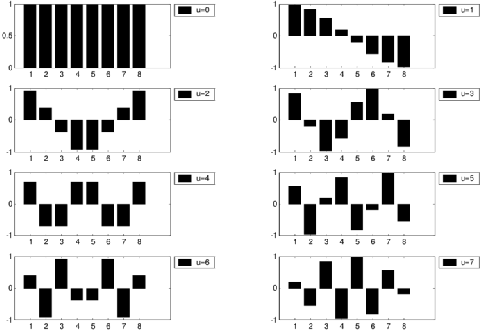
\includegraphics[width=0.8\textwidth]{slike/bazne_funkcije_1D.pdf}
\end{center}
\caption{Enodimenzionalne kosinusne bazne funkcije ($N=8$).}
\label{1D_bazne_funkcije}
\end{figure}



\section{Dvodimenzionalni DCT} % vir (https://web.archive.org/web/20150711105353/http://wisnet.seecs.nust.edu.pk/publications/tech_reports/DCT_TR802.pdf)

Idejo enodimenzionalnega DCT bomo sedaj razširili na dve dimenziji. Po želji se lahko ta metoda razširi na poljubno število dimenzij. Nas višje dimenzije ne bodo zanimale, saj se bomo kasneje osredotočili na uporabo DCT pri slikah, kjer bomo delali na dvodimenzionalnih podatkih. \par
Ta definicija je direktna razširitev enodimenzionalnega primera in sicer

\begin{equation}
    \begin{aligned}
    &C(u,v) = \alpha(u) \alpha(v) \sum_{x=0}^{N-1}\sum_{y=0}^{N-1} f(x,y)
    \cos\left[\frac{\pi(2x+1)u}{2N}\right]
    \cos\left[\frac{\pi(2y+1)u}{2N}\right], \\
    &u,v = 0,1,2,\ldots,N-1.
    \end{aligned}
\label{eq:2D-DCT}
\end{equation}
$\alpha(u)$ in $\alpha(v)$ sta enako definirana kot v \ref{eq:definicija_alpha}. Funkcija $f(x,y)$ je realna funkcija definirana na $x,y = 0,1,2,\ldots,N-1$. Inverzna transformacija je definirana kot

\begin{equation}
    \begin{aligned}
    &f(x,y) = \sum_{u=0}^{N-1}\sum_{v=0}^{N-1} \alpha(u) \alpha(v) C(u,v)
    \cos\left[\frac{\pi(2x+1)u}{2N}\right]
    \cos\left[\frac{\pi(2x+1)v}{2N}\right],  \\
    &x,y = 0,1,2,\ldots,N-1
    \end{aligned}
\label{eq:2D-DCT-inverse}
\end{equation}

Bazne funkcije za $N=8$ so prikazane v Sliki \ref{2D_bazne_funkcije}. Opazimo, da ko gremo dol po sliki se navpična frekvenca veča, ko gremo v desno se vodoravne frekvence večajo. Zgornja leva bazna funkcija je rezultat množenja komponente DC v Sliki \ref{1D_bazne_funkcije} s svojo transponirano različico. Iz tega sledi, da je ta funkcija konstantna, ki ji enako pravimo DC koeficient. Vsem ostalim podobno rečemo AC koeficienti.\par

\begin{figure}[ht] % vir (https://www.mathworks.com/help/images/discrete-cosine-transform.html)
\begin{center}
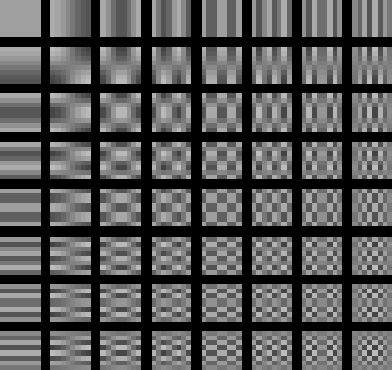
\includegraphics[width=0.6\textwidth]{slike/bazne_funkcije_2D.pdf}
\end{center}
\caption{Dvodimenzionalne bazne funkcije DCT ($N=8$). Srednja siva barva predstavlja ničelno amplitudo, svetlo siva predstavlja pozitivno in temno siva negativno amplitudo}
\label{2D_bazne_funkcije}
\end{figure}

\subsection{Separabilnost} \label{Separabilnost}% vir (https://web.archive.org/web/20150711105353/http://wisnet.seecs.nust.edu.pk/publications/tech_reports/DCT_TR802.pdf)
Eden izmed mnogih razlogov zakaj je DCT postal popularen je dejstvo, da lahko večdimenzionalne verzije DCT izračunamo z zaporednimi enodimenzionalnimi DCT-ji. Pogledali si bomo to na primeru dveh dimenzij. Definicijo dvodimenzionalne DCT \ref{eq:2D-DCT} lahko zapišemo sledeče
\begin{equation}
    \begin{aligned}
    &C(u,v) = \left(\alpha(u)  \sum_{x=0}^{N-1}\cos\left[\frac{\pi(2x+1)u}{2N}\right]
              \left(\alpha(v)  \sum_{y=0}^{N-1} f(x,y)\cos\left[\frac{\pi(2y+1)u}{2N}\right]\right)\right), \\
    &u,v = 0,1,2,\ldots,N-1.
    \end{aligned}
\label{eq:2D-DCT_Separabilnost}
\end{equation}
Ta lastnost nam omogoča, da lahko $C(u,v)$ izračunamo v dveh zaporedni enodimenzionalnih operacijah na vrsticah in stolpcih. Ideja je prikazana v Sliki \ref{Prikaz_separabilnosti}. Podobno lahko izpeljemo enačbo \ref{eq:2D-DCT-inverse} in pokažemo, da je inverzen DCT tudi separabilen.\par


\begin{figure}[ht] % vir (https://web.archive.org/web/20150711105353/http://wisnet.seecs.nust.edu.pk/publications/tech_reports/DCT_TR802.pdf)
\begin{center}
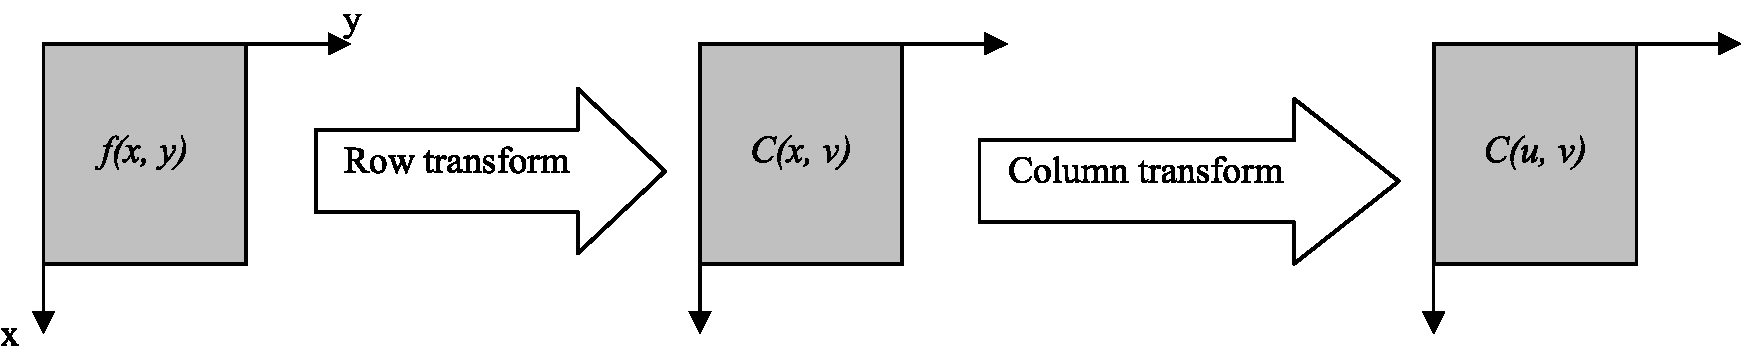
\includegraphics[width=1\textwidth]{slike/Prikaz_Separabilnosti.pdf}
\end{center}
\caption{Dvodimenzionalne bazne funkcije DCT ($N=8$). Srednja siva barva predstavlja ničelno amplitudo, svetlo siva predstavlja pozitivno in temno siva negativno amplitudo}
\label{Prikaz_separabilnosti}
\end{figure}

To lastnost bomo potrebovali pri algoritmu za hiter DCT. Ta algoritem bomo pokazali na eni dimenziji in ga nato razširili na dve dimenziji s pomočjo te lastnosti.

\section{Algoritem za hiter DCT}\label{Algoritem za hiter DCT}
V tem razdelku bomo predstavili enega izmed algoritmov za hiter izračun DCT. Povzeli bomo algoritem opisan v~\cite{FastDCT}.
Ta algoritem uporablja že obstoječe algoritme za hitro Fourierovo transformacijo(FFT) in njihove rezultate le prilagodi, da ustrezajo definiciji DCT. Obstajajo tudi alternativne izbire, ki ne uporabljajo FFT temveč rekurzivno uporabljajo različne tipe DCT-jev. Primer takšnega algoritma je opisan tudi v~\cite{britanak2010discrete}. Katero implementacijo uporabimo je odvisno kakšne so naše potrebe in zmogljivosti. Odvisno kakšne imamo strojne zmogljivosti so lahko različni algoritmi optimalni. Na primer strojne implementacije direktno na čipih uporabljajo drugačne algoritme kot pa implementaciji v programski opremi na večnamenskih procesorjih. Tukaj predstavljen algoritem je implementiran v programskem jeziku Python, v knjižnici scipy.fftpack pod imenom scipy.fftpack.dct. Tukaj bomo naredili izpeljavo, ki tesno sledi izpeljavi v~\cite{FastDCT}. Paziti moramo, saj v~\cite{FastDCT} je uporabljena nestandardna definicija za DCT, kjer je vodilni koeficient drugačen.\par
Želimo izračunati DCT od $f(x)$, ki je zaporedje realnih števil dolžine $N$, torej je definirano na $0 \leq x \leq N-1$. DCT bomo prvo izpeljali iz 2N točkovne diskretne Fourierove transformacije(DFT). Definirajmo 
\begin{equation}
  g(x)=
    \begin{cases}
          f(x), & 0 \leq x \leq N-1 \\
          f(2N-x-1), & N \leq x \leq 2N-1 \\
    \end{cases}
\label{eq:fastDCT_y}
\end{equation}

Velja $g(2N-x-1) = g(x)$.
Definirajmo DFT od $g(x)$ kot
\begin{equation}
  G(u) = \sum_{x=0}^{2N-1} g(x) W_{2N}^{xu}
\label{eq:DFT}
\end{equation}
kjer je
\begin{equation}
  W_{M} = e^{-i2\pi/M}.
\label{eq:DFT_W}
\end{equation}

Če zamenjamo \ref{eq:fastDCT_y} v \ref{eq:DFT} dobimo
\begin{equation}
  G(u) = \sum_{x=0}^{N-1} f(x) W_{2N}^{xu} + \sum_{x=N}^{2N-1} x(2N-x-1) W_{2N}^{xu}.
\label{eq:DFT_z_g1}
\end{equation}
V desni vsoti uporabimo novo spremenljivko vsote in upoštevamo, da je $W_{2N}^{2mN} = 1$ za $\forall m \in \mathbb{Z}$. Izpostavimo $W_{2N}^{-u/2}$ in dobimo
\begin{equation}
  G(u) = W_{2N}^{-u/2}\sum_{x=0}^{N-1} f(x) \left[ W_{2N}^{xu}W_{2N}^{u/2} + W_{2N}^{-xu}W_{2N}^{-u/2} \right].
\label{eq:DFT_z_g2}
\end{equation}
Izraz v \ref{eq:DFT_z_g2} lahko zapišemo na dva načina
\begin{equation}
  G(u) = W_{2N}^{-u/2} 2 \sum_{x=0}^{N-1} f(x) \cos\frac{\pi(2x+1)u}{2N}, \indent 0 \leq u \leq 2N-1
\label{eq:DFT_z_enacbo_DCT}
\end{equation}

ali

\begin{equation}
  G(u) = W_{2N}^{-u/2} 2 Re \left[ W_{2N}^{u/2} \sum_{x=0}^{N-1} f(x) W_{2N}^{xu} \right], \indent 0 \leq u \leq 2N-1
\label{eq:DFT_z_Re}
\end{equation}
kjer $Re$ pomeni, da vzamemo realno komponento kompleksnega števila.
Vstavimo definicijo DCT iz \ref{eq:1D-DCT} v \ref{eq:DFT_z_enacbo_DCT} in dobimo

\begin{equation}
  G(u) = W_{2N}^{-u/2} \frac{2}{\alpha(u)} C(u)
\label{eq:DFT_z_DCT}
\end{equation}
ali
\begin{equation}
  C(u) = W_{2N}^{u/2} \frac{\alpha(u)}{2} G(u)
\label{eq:DCT_z_DFT}
\end{equation}
Vstavimo \ref{eq:DFT_z_Re} v \ref{eq:DCT_z_DFT} dobimo

\begin{equation}
  G(u) = \alpha(u) Re \left[ W_{2N}^{u/2} \sum_{x=0}^{N-1} f(x) W_{2N}^{xu} \right], \indent 0 \leq u \leq 2N-1
\label{eq:DCT_z_Re}
\end{equation}
V \ref{eq:DCT_z_Re} vidimo, da lahko DCT od $f(x)$ dobimo tako, da izračunamo 2N točkovni DFT originalnega f(x) z N ničlami dodanimi na koncu. Nato pomnožimo rezultat s $W_{2N}^{u/2}$, vzamemo realni del tega in pomnožimo z $\alpha(u)$.\par
Sedaj potrebujemo še hiter inverzni DCT. Tega izpeljemo na podoben način, kjer prvo vzamemo inverzni DFT. Inverzni DFT od $G(u)$ je definiran kot 
\begin{equation}
  G(u) = \frac{1}{2N}\sum_{u=0}^{2N-1} G(u) W_{2N}^{-xu}.
\label{eq:Inverse_DFT}
\end{equation}
Ker je $g(x)$ realna funkcija je posledično njen DFT $G(x)$ Hermitsko simetričen, torej
\begin{equation}
  G(2N - u) = G\text{*}(u).
\label{eq:Hermitska_simetricnost}
\end{equation}
Potrebujemo tudi, da po \ref{eq:DFT_z_Re} velja
\begin{equation}
  G(N) = 0.
\label{eq:G(N)=0}
\end{equation}
Če vstavimo \ref{eq:Hermitska_simetricnost} in \ref{eq:G(N)=0} v \ref{eq:Inverse_DFT} dobimo 
\begin{equation}
  g(x) = \frac{1}{N} Re \left[ \frac{G(0)}{2} + \sum_{u=1}^{N-1} G(u) W_{2N}^{-xu}   \right], \indent 0 \leq x \leq 2N-1
\label{eq:Inverse_DCT_z_DFT}
\end{equation}
Če vstavimo \ref{eq:DFT_z_DCT} v \ref{eq:Inverse_DCT_z_DFT} in uporabimo \ref{eq:fastDCT_y} dobimo inverzni DCT kot zapisan v \ref{eq:1D-DCT-inverse}.\par
Torej če imamo dan $C(u)$ dobimo $f(x)$ tako, da prvo izračunamo $G(u)$ po \ref{eq:DFT_z_DCT}. Nato s pomočjo \ref{eq:Inverse_DCT_z_DFT} dobimo $g(x)$ in iz njega pridobimo $f(x)$ po \ref{eq:fastDCT_y}.





\begin{comment}
V~\cite{FastDCT} je izpeljano, da lahko zapišemo DCT od $f(x)$ kot
\begin{equation}
  C(u) = \alpha(u) Re \left[ W_{4N}^{u} \sum_{x=0}^{N-1} v(x) W_N^{xu}\right], \indent 0 \leq u \leq N-1
\label{eq:DCT_z_DFT_Dolzine_N}
\end{equation}
Tukaj vidimo da je $\sum_{x=0}^{N-1} v(u) W_N^{xu}$ DFT od $v(u)$ z $N$ točkami, kar se bo izračunalo s hitrim algoritmom za DFT, ki se mu reče FFT. Kasneje bomo zapisali psevdokodo algoritma FFT.\par

Sedaj izračunajmo še inverzni DCT s pomočjo inverznega DFT.

\begin{equation}
  v(u) = \frac{1}{N} \sum_{x=0}^{N-1} V(u) W_{N}^{-xu}
\label{eq:inverse_DFT}
\end{equation}

Po izpeljavi v~\cite{FastDCT} je najprej potrebno izračunati $V(u)$ kot


\begin{equation}
  V(u) = \frac{1}{2} W_{4N}^{-u}\left[ C(u) - iC(N-u) \right], \indent 0 \leq u \leq N-1
\label{eq:izracun_V}
\end{equation}
V tej definiciji 

% potrebno pokazat, da lahko izračunamo DCT z (N/2) kompleksnim IDFT. To se naredi tako da se uporabi hermetsko simetrično zaporedja.(zapisano v Appendix od članka)!!!!!!!!!!!!!!!!!!!!


    

\begin{equation}
  v(x)=
    \begin{cases}
          f(2x), & 0 \leq x \leq \lfloor\frac{N-1}{2}\rfloor \\
          f(2N-2x-1), & \lfloor\frac{N+1}{2}\rfloor \leq x \leq N-1 \\
    \end{cases}
\label{eq:fastDCT_v}
\end{equation}
Ta definicija pravi, da najprej vzamemo sode točke $f(x)$ po vrsti in za njimi lihe točke v obratnem vrstnem redu.
\end{comment}


\section{Integer DCT}
Prikazali bomo eno metodo aproksimacije DCT s celimi števili. To je zaželeno zaradi bolj enostavne aritmetike pri računanju s celimi števili. Implementacijo, ki si bomo ogledali tukaj je z množenjem in seštevanje celih števil. Obstajajo sicer tudi implementacije, ki uporabljajo zgolj binarno seštevanje in operacijo bit shift. Tukaj se lahko običajno dosežejo boljši rezultati v primeru, da uporabljamo števila z več biti. Posledično se sicer poveča računska zahtevnosti. Predstavili bomo eno izmed bolj enostavnih implementacij celoštevilskega DCT, ki je opisana v~\cite{britanak2010discrete}. Ista knjiga vsebuje tudi bolj napredne implementacije v katere se tukaj ne bomo poglabljali.\par
Pokazali bomo korake kako pretvoriti realno številski DCT v celoštevilski DCT. Tukaj si bomo ogledali samo primer, ko je $N=8$, zaradi enostavnosti razlage. V splošnem je ta primer tudi najbolj pogosto uporabljan. Torej želeli bomo aproksimirati DCT matriko $C_8$, ki smo jo definirali v \ref{eq:1D_DCT_matrika}, z $\widetilde{C_8}$. $\widetilde{C_8}$ bo definirana kot
\begin{equation}
  \widetilde{C_8} = Q_8 V_8
\label{eq:c_8}
\end{equation}
V tem zapisu $Q_8$ predstavlja diagonalno matriko z normalizacijskimi faktorji na glavni diagonali. Ti niso nujno celoštevilki, potrebujemo jih, da bo naša DCT ortonormirana. Postopek pridobitve $\widetilde{C_8}$ iz $C_8$ je sledeč.
Najprej bomo generirali $C_8$ v ekspicitni in numerični obliki
\begin{gather*}
 C_8 = \frac{1}{2}
  \setlength{\arraycolsep}{1pt}
  \renewcommand{\arraystretch}{1}
  \begin{bmatrix}
  \frac{1}{\sqrt{2}} & \frac{1}{\sqrt{2}} & \frac{1}{\sqrt{2}} & \frac{1}{\sqrt{2}} & \frac{1}{\sqrt{2}} & \frac{1}{\sqrt{2}} & \frac{1}{\sqrt{2}} & \frac{1}{\sqrt{2}}\\
  \cos{\frac{\pi}{16}} & \cos{\frac{3\pi}{16}} & \sin{\frac{3\pi}{16}} & \sin{\frac{\pi}{16}} & -\sin{\frac{\pi}{16}} & -\sin{\frac{3\pi}{16}} & -\cos{\frac{3\pi}{16}} & -\cos{\frac{\pi}{16}}\\
  \cos{\frac{\pi}{8}} & \sin{\frac{\pi}{8}} & -\sin{\frac{\pi}{8}} & -\cos{\frac{\pi}{8}} & -\cos{\frac{\pi}{8}} & -\sin{\frac{\pi}{8}} & \sin{\frac{\pi}{8}} & \cos{\frac{\pi}{8}} \\
  \cos{\frac{3\pi}{16}} & -\sin{\frac{\pi}{16}} & -\cos{\frac{\pi}{16}} & -\sin{\frac{3\pi}{16}} & \sin{\frac{3\pi}{16}} & \cos{\frac{\pi}{16}} & \sin{\frac{\pi}{16}} & -\cos{\frac{3\pi}{16}}\\
  \frac{1}{\sqrt{2}} & -\frac{1}{\sqrt{2}} & -\frac{1}{\sqrt{2}} & \frac{1}{\sqrt{2}} & \frac{1}{\sqrt{2}} & -\frac{1}{\sqrt{2}} & -\frac{1}{\sqrt{2}} & \frac{1}{\sqrt{2}}\\
  \sin{\frac{3\pi}{16}} & -\cos{\frac{\pi}{16}} & \sin{\frac{\pi}{16}} & \cos{\frac{3\pi}{16}} & -\cos{\frac{3\pi}{16}} & -\sin{\frac{\pi}{16}} & \cos{\frac{\pi}{16}} & -\sin{\frac{3\pi}{16}}\\
  \sin{\frac{\pi}{8}} & -\cos{\frac{\pi}{8}} & \cos{\frac{\pi}{8}} & -\sin{\frac{\pi}{8}} & -\sin{\frac{\pi}{8}} & \cos{\frac{\pi}{8}} & -\cos{\frac{\pi}{8}} & \sin{\frac{\pi}{8}} \\
  \sin{\frac{\pi}{16}} & -\sin{\frac{3\pi}{16}} & \cos{\frac{3\pi}{16}} & -\cos{\frac{\pi}{16}} & \cos{\frac{\pi}{16}} & -\cos{\frac{3\pi}{16}} & \sin{\frac{3\pi}{16}} & -\sin{\frac{\pi}{16}}\\
   \end{bmatrix}
\end{gather*}

\begin{gather*}
   =
 \setlength{\arraycolsep}{1pt}
 \renewcommand{\arraystretch}{1}
 \begin{bmatrix}
    0.3535&  0.3535&  0.3535&  0.3535&  0.3535&  0.3535&  0.3535&  0.3535\\
    0.4903&  0.4157&  0.2777&  0.0975& -0.0975& -0.2777& -0.4157& -0.4903\\
    0.4619&  0.1913& -0.1913& -0.4619& -0.4619& -0.1913&  0.1913&  0.4619\\
    0.4157& -0.0975& -0.4903& -0.2777&  0.2777&  0.4903&  0.0975& -0.4157\\
    0.3535& -0.3535& -0.3535&  0.3535&  0.3535& -0.3535& -0.3535&  0.3535\\
    0.2777& -0.4903&  0.0975&  0.4157& -0.4157& -0.0975&  0.4903& -0.2777\\
    0.1913& -0.4619&  0.4619& -0.1913& -0.1913&  0.4619& -0.4619&  0.1913\\
    0.0975& -0.2777&  0.4157& -0.4903&  0.4903& -0.4157&  0.2777& -0.0975\\
 \end{bmatrix}
\end{gather*}
Označimo s $c_{ij}$ koeficiente tabele $C_8$. Če gledamo absolutne vrednosti elementov $C_8$ vidimo sledeče
\begin{alignat*}{1}
    & |c_{00}| = |c_{01}| = |c_{02}| = |c_{03}| = |c_{04}| = |c_{05}| = |c_{06}| = |c_{07}| = \\
    &  = |c_{40}| = |c_{41}| = |c_{42}| = |c_{43}| = |c_{44}| = |c_{45}| = |c_{46}| = |c_{47}| = \frac{1}{\sqrt{2}},\\
    & |c_{10}| = |c_{17}| = |c_{32}| = |c_{35}| = |c_{51}| = |c_{56}| = |c_{73}| = |c_{74}| = \cos{\frac{\pi}{16}},\\
    & |c_{11}| = |c_{16}| = |c_{30}| = |c_{37}| = |c_{53}| = |c_{54}| = |c_{72}| = |c_{75}| = \cos{\frac{3\pi}{16}},\\
    & |c_{12}| = |c_{15}| = |c_{33}| = |c_{34}| = |c_{50}| = |c_{57}| = |c_{71}| = |c_{76}| = \sin{\frac{3\pi}{16}},\\
    & |c_{13}| = |c_{14}| = |c_{31}| = |c_{36}| = |c_{52}| = |c_{55}| = |c_{70}| = |c_{77}| = \sin{\frac{\pi}{16}},\\
    & |c_{20}| = |c_{23}| = |c_{24}| = |c_{27}| = |c_{61}| = |c_{62}| = |c_{65}| = |c_{66}| = \cos{\frac{\pi}{8}},\\
    & |c_{21}| = |c_{22}| = |c_{25}| = |c_{26}| = |c_{60}| = |c_{63}| = |c_{64}| = |c_{67}| = \sin{\frac{\pi}{8}}.
\end{alignat*}
Vidimo, da je v $C_8$ le 7 različnih vrednosti. Zapišemo elemente z enako magnitudo z isto spremenljivko iz množice $\{a,b,c,d,e,f,g\}$, kjer so $a,b,c,d,e,f,g \in \mathbb{N}$. Definirajmo $V_8$ tako, da ohranimo istoležne predznake od $C_8$ in na mestih, kjer ima $C_8$ števila enake magnitude dajmo isto spremenljivko. Izrazimo $\widetilde{C_8}$ po tej definiciji.
\begin{gather}
   \widetilde{C_8} = Q_8
 \begin{bmatrix}
    g&  g&  g&  g&  g&  g&  g&  g\\
    a&  b&  c&  d& -d& -c& -b& -a\\
    e&  f& -f& -e& -e& -f&  f&  e\\
    b& -d& -a& -c&  c&  a&  d& -b\\
    g& -g& -g&  g&  g& -g& -g&  g\\
    c& -a&  d&  b& -b& -d&  a& -c\\
    f& -e&  e& -f& -f&  e& -e&  f\\
    d& -c&  b& -a&  a& -b&  c& -d\\
 \end{bmatrix}
\label{eq:IntegerDCT_Q8}
\end{gather}
Želimo, da sta i-ti in j-ti bazni vektor ortogonalna. Označimo i-to in j-to vrstico $V_8$ kot $v_i$ in $v_j$. Ta vektorja sta ortogonalna, če je njun skalarni produkt 0 torej
\begin{equation*}
    v_i v_j^T = \sum_{k=0}^7v_{ik}v_{kj} = 0,\indent \forall i \neq j, \indent i,j = 0,1,\ldots,
\end{equation*}

Za ortonormalnost potrebujemo še, da je norma stolpcev $\widetilde{C_8}$ enaka 1. Najprej definirajmo drugo normo baznega vektorja
\begin{equation}
    \lVert v_i \rVert_2 = \sqrt{\sum_{k=0}^7 v_{ik}^2}, \indent i,k = 0,1,\ldots,7
\end{equation}
Definirajmo še 
\begin{equation}
    q_{ii} = \lVert v_i \rVert_2^2.
\end{equation}
Sedaj lahko definiramo matriko $Q_8$ kot
\begin{equation}
    Q_8 = diag\left(\frac{1}{\sqrt{q_{00}}},\ldots,\frac{1}{\sqrt{q_{77}}}\right).
\end{equation}
Ta definicija zagotovi, da bo $\widetilde{C_8}$ ortonormalna. Členi $\frac{1}{\sqrt{q_{ii}}}$ so v splošnem iracionalna števila. Temu se ne moramo izogniti, če želimo imeti ortonormalni DCT. Pogoj za ortogonalnost lahko zapišemo tudi kot
\begin{equation}
    V_8 V_8^T = [Q_8^{-1}]^2I_8.
\end{equation}
Iz tega pogoja pridobimo enačbo
\begin{equation}
    a(b-c)-d(b+c) = 0
\label{eq:integerDCT_pogoj}
\end{equation}
in
\begin{equation}
  \begin{aligned}
    &q_{00} = q_{44} = 8g^2\\
    &q_{11} = q_{33} = q_{55} = q_{77} = 2(a^2 + b^2 + c^2 + d^2)\\
    &q_{22} = q_{66} = 4(e^2 + f^2)
  \end{aligned}
\label{eq:integerDCT_q_ii}
\end{equation}
Iz teh pogojev vidimo, da lahko spremenljivke $e$, $f$ in $g$ obravnavamo ločeno od $a$, $b$, $c$ in $d$.\par
Določiti moramo še nekaj neeneakosti med temi koeficienti, da bodo magnitude baznih vektorjev $V_8$ približno enako tistim v matriki $C_8$. Z upoštevanjem \ref{eq:integerDCT_pogoj} in \ref{eq:integerDCT_q_ii} lahko določimo sledeče neenakosti
\begin{align} 
  \label{eq:integerDCT_neenakost_1}
  &a > b > c > d > 0, \\
  \label{eq:integerDCT_neenakost_2}
  &a > e > f > 0, \\
  \label{eq:integerDCT_neenakost_3}
  &a > g > 0.
\end{align}
Želimo najti množico celih števil $\{a,b,c,d,e,f,g\}$, ki zadoščajo enakosti \ref{eq:integerDCT_pogoj} in neenakostim \ref{eq:integerDCT_neenakost_1}-\ref{eq:integerDCT_neenakost_3}. Za rešitev te enačbe lahko iščemo števila v množici $\{a,b,c,d,e,f,g\}$, ki so predstavljena z $M$ biti. V splošnem je tukaj lahko neskončno rešitev enačbe s temi omejitvami. DCT s celimi števili je določena s $\{a,b,c,d,e,f,g\}$, kar bomo označili kot $IntegerDCT_8(a,b,c,d,e,f,g)$. Izbrano množico $\{a,b,c,d,e,f,g\}$ bomo vstavili v matriko $V_8$ kot definirano v \ref{eq:IntegerDCT_Q8}. Podobno vstavimo vse $q_{ii}$ dane v \ref{eq:integerDCT_q_ii} vstavimo v $Q_8$. Vse rešitve, ki upoštevajo enačbo \ref{eq:integerDCT_pogoj} in omejitve \ref{eq:integerDCT_neenakost_1}-\ref{eq:integerDCT_neenakost_3} nam bodo dalo matriko $\widetilde{C_8}$, ki je ortonormalna in blizu matriki $C_8$. Efektivnost implementacije $IntegerDCT_8(a,b,c,d,e,f,g)$ bo odvisna predvsem od izbire velikosti koeficientov, torej kako velik $M$ bomo dovolili.\par
Tukaj bomo povedali nekaj primerov, ko bodo $e=3$, $g=1$ in $f =1$. To je izbira opisana v~\cite{britanak2010discrete}. Torej pogledali si bomo nekaj primerov $IntegerDCT_8(a,b,c,d,3,1,1)$, kjer bomo za M vzeli vrednosti 3, 4, 5, 6, 7 ali 8. Za mero točnosti specifičnega približka bomo pa uporabili mero srednje kvadratne napake, ki jo označimo z MSE(\textit{Mean squared error}) in je definirana kot
\begin{equation} % moram nekje najdit da bom citiral tako verzijo definicije
  MSE = \frac{1}{n}\sum_{i=0}^{i=n-1}\sum_{j=0}^{j=m-1}\left(X_{ij} - \widetilde{X_{ij}} \right)^2.
\label{eq:MSE}
\end{equation}
Tukaj je $X$ originalna matrika in $\widetilde{X}$ približek originalni matriki.\par
Primerjali bomo MSE različnih $IntegerDCT_8(a,b,c,d,3,1,1)$ v primerjavi z originalnim DCT v Tabeli \ref{tab:IntegerDCT_8}

\begin{table}[ht]
\centering
\begin{tabular}{|l|c|}
\hline
$IntegerDCT_8(a,b,c,d,3,1,1)$              &MSE          \\
\hline
$DCT                                     $ &0             \\
$IntegerDCT_8(5, 3, 2, 1, 3, 1, 1)       $ &2.721681e-003\\ 
$IntegerDCT_8(7, 4, 3, 1, 3, 1, 1)       $ &3.006062e-003\\ 
$IntegerDCT_8(10, 9, 6, 2, 3, 1, 1)      $ &2.060647e-004\\ 
$IntegerDCT_8(14, 12, 9, 2, 3, 1, 1)     $ &4.691150e-004\\ 
$IntegerDCT_8(12, 10, 6, 3, 3, 1, 1)     $ &4.154884e-004\\ 
$IntegerDCT_8(15, 12, 8, 3, 3, 1, 1)     $ &2.059246e-004\\ 
$IntegerDCT_8(24, 21, 15, 4, 3, 1, 1)    $ &2.914385e-004\\ 
$IntegerDCT_8(25, 21, 14, 5, 3, 1, 1)    $ &1.302862e-004\\ 
$IntegerDCT_8(25, 24, 16, 5, 3, 1, 1)    $ &4.693343e-004\\ 
$IntegerDCT_8(26, 24, 15, 6, 3, 1, 1)    $ &2.913951e-004\\ 
$IntegerDCT_8(45, 39, 26, 9, 3, 1, 1)    $ &1.380974e-004\\ 
$IntegerDCT_8(45, 42, 28, 9, 3, 1, 1)    $ &3.317750e-004\\ 
$IntegerDCT_8(55, 51, 34, 11, 3, 1, 1)   $ &3.049383e-004\\ 
$IntegerDCT_8(55, 48, 32, 11, 3, 1, 1)   $ &1.458331e-004\\ 
$IntegerDCT_8(65, 57, 38, 13, 3, 1, 1)   $ &1.524257e-004\\ 
$IntegerDCT_8(75, 66, 44, 15, 3, 1, 1)   $ &1.578933e-004\\ 
$IntegerDCT_8(85, 75, 50, 17, 3, 1, 1)   $ &1.624316e-004\\ 
$IntegerDCT_8(120, 105, 70, 24, 3, 1, 1) $ &1.492797e-004\\ 
$IntegerDCT_8(175, 153, 102, 35, 3, 1, 1)$ &1.481648e-004\\ 
$IntegerDCT_8(185, 162, 108, 37, 3, 1, 1)$ &1.503612e-004\\ 
$IntegerDCT_8(230, 201, 134, 46, 3, 1, 1)$ &1.475946e-004\\ 
$IntegerDCT_8(250, 219, 146, 50, 3, 1, 1)$ &1.508895e-004\\
\hline
\end{tabular}
\caption{Tabela različnih možnih $IntegerDCT_8(a,b,c,d,3,1,1)$ s pripadajočimi MSE od originalnega DCT}
\label{tab:IntegerDCT_8}
\end{table}
Izpišimo še en primer tabele $\widetilde{C_8}$ za primer $IntegerDCT_8(15, 12, 8, 3, 3, 1, 1)$

\begin{gather}
   \widetilde{C_8} = Q_8
 \begin{bmatrix}
    1&    1&   1&    1&   1&   1&    1&   1\\
    15&  12&   8&    3&  -3&  -8&  -12& -15\\
    3&    1&  -1&   -3&  -3&  -1&   1&    3\\
    12&  -3& -15&   -8&   8&  15&   3&  -12\\
    1&   -1&  -1&    1&   1&  -1&  -1&    1\\
    8&  -15&   3&   12& -12&  -3&  15&   -8\\
    1&   -3&   3&   -1&  -1&   3&  -3&    1\\
    3&   -8&   12& -15&  15& -12&   8&   -3\\
 \end{bmatrix}
\label{eq:IntegerDCT_8(15, 12, 8, 3, 3, 1, 1)}
\end{gather}
kjer so $q_{ii}$ dani kot
\begin{equation}
  \begin{aligned}
    &q_{00} = q_{44} = 1\\
    &q_{11} = q_{33} = q_{55} = q_{77} = 884\\
    &q_{22} = q_{66} = 10
  \end{aligned}
\end{equation}
torej je
\begin{equation}
    Q_8 = diag\left(\frac{1}{\sqrt{8}}, \frac{1}{\sqrt{442}},\frac{1}{\sqrt{40}},\frac{1}{\sqrt{442}},\frac{1}{\sqrt{8}},\frac{1}{\sqrt{442}},\frac{1}{\sqrt{40}},\frac{1}{\sqrt{442}}, \right).
\end{equation}
Tukaj smo zapisali samo matriko s katero bi morali množiti vektor vrednosti signala, da bi dobili DCT. V knjigi~\cite{britanak2010discrete} so zapisane še izboljšave tega algoritma in opisan je tudi način kako lahko tak DCT izračunamo v podobnem številu korakov kot smo pokazali pri hitri verziji navadnega DCT.















\chapter{Implementacije DCT za slike}
\label{ch2}

\section{JPEG}
\subsection{Uvod v JPEG}
Format JPEG je izdan v standardu ISO/IEC 10918. Ime dobi od skupine, ki ga je ustvarila, ki se imenuje Joint Photographic Experts Group. Izdan je bil leta 1992.\par
JPEG standard določa zgolj ogrodje formata, ki poda nekatere zahteve in predloge za uporabo. Ponuja veliko število opcijskih implementacij, ki so odvisne od namenjene uporabe in od potrebe po moči kompresije. Tukaj bomo predstavili podrobneje zgolj eno izmed bolj popularnih izvedb uporabe tega formata.\par 

JPEG podpira štiri različne načine delovanja. Prve trije od teh uporabljajo kompresijo z izgubo in zadnja uporablja kompresijo brez izgub.
\begin{itemize}
   \item Zaporedno kodiranje (\textit{Sequential encoding}): slika je kodirana od leve proti desni in od vrha do dna.
   \item Progresivno kodiranje (\textit{Progressive encoding}): slika je kodirana v več obhodih za aplikacije, kjer je čas prenosa dolg. Tukaj ob dekodiranju takoj dobimo nizko resolucijo slike, ki z obhodi pridobiva na ločljivosti.
   \item Hierarhično kodiranje (\textit{Hierarchical encoding}): slika je kodirana pri več različnih resolucijah. Na ta način lahko dostopamo do nižjih resolucij brez da bi morali dekompresirati slika pri polni resoluciji.
   \item Kodiranje brez izgub (\textit{Lossless encoding}): slika je kodirana, da ob dekodiranju dobimo identično kopijo originala (ta način delovanja, da zelo minimalno kompresijo)
\end{itemize}
Vsak od teh načinov delovanja ima kasneje še specificiranih več različnih kodekov (par kodirnika in dekodirnika).
Od sedaj naprej bomo govorili zgolj o zaporednem kodiranju, saj je to najpogostejša implementacija v današnjih programih.\par
\subsection{Predprocesiranje}
Osnovni format JPEG sam po sebi ne določi veliko o barvnih kanalih. Lahko ga uporabljamo za slike v sivinah(\textit{grayscale images}), kar je najbolj enostaven primer, saj tu imamo zgolj en barvni kanal. V tem primeru se ta barvni kanal lahko direktno pošlje dalje. Bolj pogosto se uporabljajo barvne slike. Te imajo običajno tri barvne kanale. Najpogostejši od teh zapisov je v oblike RGB, kjer imamo po en kanal za rdečo, zeleno in modro intenziteto. Te bi lahko obravnavali kot neodvisne in jih ločeno poslali dalje ter jih šele ob dekodiranju nazaj združili. Bolj uspešen način za višjo kompresijo je, da jih preslikamo v barvni prostor, kjer se loči svetilnost (\textit{luminance}) in barvo (\textit{chrominance}). Torej bomo iz RGB prostora preslikali v prostor Y'C\textsubscript{B}C\textsubscript{R}, kjer Y' predstavlja svetilnost, medtem ko C\textsubscript{B} in C\textsubscript{R} predstavljata barvo. To naredimo, ker je človeško oko bolj občutljivo na svetilnost kot na barvo. Nato bomo izvedli chroma subsampling preden pošljemo sliko dalje. Najpogosteje se uporablja chroma subsampling 4:2:2 ali 4:2:0. Prvi iz barvnih kanalov odstrani $1/2$ podatkov torej, če gledamo celotne podatke tu odstranimo $1/3$. V drugem primeru odstranimo $3/4$ barvnih podatkov, torej v celoti $1/2$ podatkov. Tu se zmanjša resolucija drugih dveh kanalov, ko jih pošljemo dalje. \par
% vir za chroma subsampling https://www.researchgate.net/publication/321286841_Chroma_Subsampling_Influence_on_the_Perceived_Video_Quality_for_Compressed_Sequences_in_High_Resolutions

Preden razdelimo sliko na bloke je potrebno dodat dovolj pikslov, da bo število pikslov v vodoravni in navpični smeri deljivo z 8. Kako se to naredi ni specificirano v standardu. Ena od pogostejših metod je, da zrcalimo najbolj robne piksle (\textit{Reflection padding}). Nato razdelimo sliko na bloke velikosti 8x8. Označimo vrednosti v teh blokih z $f(x,y)$, kjer je $x,y = 0,1,2,\ldots,7$. Izbira velikosti bloka je 8x8, zaradi hitre izračunljivosti in hkrati dobimo zelo dobre rezultate pri kompresiji in vizualni ločljivosti slik. V teh blokih nato vrednosti zamaknemo iz nepredznačenih celih števil na intervalu $\left[0,2^P-1\right]$ v predznačena cela števila na interval$\left[-2^{P-1},2^{P-1}-1\right]$, kjer $P$ označuje število bitov, ki predstavljajo intenziteto piksla v tem barvnem kanalu. Običajno je $P=8$.

\subsection{Kodiranje}

Na sliki \ref{Shema_JPEG} je prikazana osnovna shema kodiranja slike v JPEG formatu.
\begin{figure}[ht] % vir (https://www.w3.org/Graphics/JPEG/itu-t81.pdf)
\begin{center}
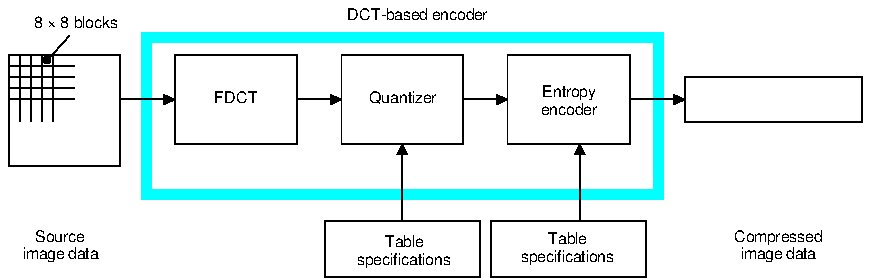
\includegraphics[width=0.9\textwidth]{slike/Shema_JPEG.pdf}
\end{center}
\caption{Shema delovanja JPEG}
\label{Shema_JPEG}
\end{figure}

Sedaj gre tak 8x8 blok skozi DCT, torej uporabi se formula \ref{eq:2D-DCT} kjer je $N=8$. Poenostavljeno zapisano sledeče
\begin{equation}
    \begin{aligned}
    &C(u,v) = \alpha(u) \alpha(v) \sum_{x=0}^{7}\sum_{y=0}^{7} f(x,y)
    \cos\left[\frac{\pi(2x+1)u}{16}\right]
    \cos\left[\frac{\pi(2y+1)u}{16}\right], \\
    &u,v = 0,1,2,\ldots,7.
    \end{aligned}
\label{eq:2D-DCT_JPEG}
\end{equation}
\begin{equation}
\alpha(u)=
    \begin{cases}
          \sqrt{\frac{1}{8}} & \text{za $u=0$} \\
          \sqrt{\frac{1}{4}} & \text{za $u\neq 0$} \\
    \end{cases}
\label{eq:definicija_alpha_JPEG}
\end{equation}
V praksi se uporabijo hitrejše metode za izračun DCT kot na primer algoritem, ki smo ga predstavili v poglavju \ref{Algoritem za hiter DCT}. V formatu JPEG ni predpisan specifičen način izračuna DCT, saj so pri različnih aplikacij različne implementacije optimalne. Različne implementacije sicer lahko privedejo do različnih rezultatov. Iz tega razloga zahtevajo le, da je algoritem znotraj mer njihovega testa natančnosti. \par
Drugi večji korak je kvantizacija (\textit{quantization}) izhoda DCT. Tukaj so vsi elementi kvantizirani s pomočjo kvantizacijske tabele velike 8x8, ki je specificirana od uporabnika ali aplikacije. Elementi te tabele so cela števila med 1 in 255, ki določijo koliko se kvantizira pripadajoč DCT koeficient. Kvantizirani koeficienti so izračunani s pomočjo naslednje formule
\begin{equation}
C^Q(u,v) = Integer \; round \left(\frac{C(u,v)}{Q(u,v)} \right)
\label{eq:kvantizacija}
\end{equation}
Ta korak je glavni vir izgube znotraj JPEG-a. Iz tega razloga je kompresija končne slike odvisna predvsem od izbire kvantizacijskih tabel. Primer takšnih tabel je podan v originalni dokumentaciji za JPEG. Tam so kot izbiro podali Tabelo \ref{tab:Kvantizacija_svetilnost} za svetilnost in Tabelo \ref{tab:Kvantizacija_barva} za barvo. Opazimo, da sta sicer tabeli različni vendar obe temeljita na principu, da se števila, ko gremo desno in navzdol višajo. Tabele so tako zgrajene ker nam podatki desno in spodaj predstavljajo bazne funkcije z višjimi frekvencami. Te so manj pomembne za vizualno ločljivost in s tem njihov pomen zmanjšamo.
\begin{table}[ht]
\centering
\begin{tabular}{|m{18pt}|m{18pt}|m{18pt}|m{18pt}|m{18pt}|m{18pt}|m{18pt}|m{18pt}|}
\hline
16& 11& 10& 16&  24&  40&  51& 61\\  \hline
12& 12& 14& 19&  26&  58&  60& 55\\  \hline
14& 13& 16& 24&  40&  57&  69& 56\\  \hline
14& 17& 22& 29&  51&  87&  80& 12\\  \hline
18& 22& 37& 56&  68& 109& 103& 77\\  \hline
24& 35& 55& 64&  81& 104& 113& 92\\  \hline
49& 64& 78& 87& 103& 121& 120& 101\\ \hline
72& 92& 95& 98& 112& 100& 103& 99\\  \hline

\end{tabular}
\caption{kvantizacijska tabela za svetilnost}
\label{tab:Kvantizacija_svetilnost}
\end{table}

\begin{table}[ht]
\centering
\begin{tabular}{|m{18pt}|m{18pt}|m{18pt}|m{18pt}|m{18pt}|m{18pt}|m{18pt}|m{18pt}|}
\hline
17& 18& 24& 47& 99& 99& 99& 99 \\ \hline
18& 21& 26& 66& 99& 99& 99& 99 \\ \hline
24& 26& 56& 99& 99& 99& 99& 99 \\ \hline
47& 66& 99& 99& 99& 99& 99& 99 \\ \hline
99& 99& 99& 99& 99& 99& 99& 99 \\ \hline
99& 99& 99& 99& 99& 99& 99& 99 \\ \hline
99& 99& 99& 99& 99& 99& 99& 99 \\ \hline
99& 99& 99& 99& 99& 99& 99& 99 \\ \hline
\end{tabular}
\caption{kvantizacijska tabela za barvo}
\label{tab:Kvantizacija_barva}
\end{table}
Kvantizacijske tabele se shranijo v glavi JPEG-a, saj se bodo kasneje potrebovale za dekodiranje.\par

Po kvantizaciji se DC koeficient kodira ločeno od 63 AC koeficientov. To se stori, ker so pogosto DC koeficienti sosednjih blokov korelirani. Kvantizirani DC koeficienti so kodirani kot razlika prejšnjega DC koeficienta in tega, kot je prikazano na Sliki \ref{Diferencialno_kodiranje_DC}. Pri prvem bloku se prejšnji koeficent šteje kot da je 0, kar je povprečna vrednost, saj smo vhodne vrednosti centrirali okoli 0.
\begin{figure}[ht] % vir (https://www.ijg.org/files/Wallace.JPEG.pdf)
\begin{center}
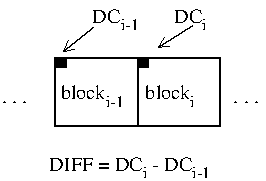
\includegraphics[width=0.3\textwidth]{slike/Diferencialno_kodiranje_DC.pdf}
\end{center}
\caption{Diferencialno DC kodiranje}
\label{Diferencialno_kodiranje_DC}
\end{figure}
Obravnavanje DC koeficientov ločeno je smiselno, ker vsebujejo večino informacij na sliki. \par
Preostanejo AC koeficienti, ki jih najprej preuredimo v enovrstično zaporedje po principu prikazanem na Sliki \ref{zig_zag_zaporedje}. S to razporeditvijo skupaj združimo koeficiente, ki predstavljajo nižje frekvence. Koeficienti na začetku zaporedja imajo večjo verjetnost, da so neničelni. To je koristno za entropijsko kodiranje (\textit{entropy coding}), ki ga bomo izvedli na teh zaporedjih.\par
\begin{figure}[ht] % vir (https://www.ijg.org/files/Wallace.JPEG.pdf)
\begin{center}
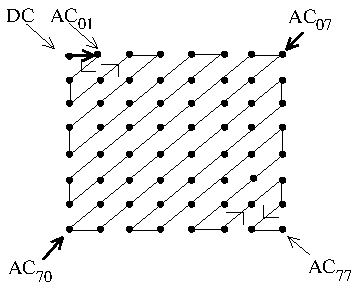
\includegraphics[width=0.5\textwidth]{slike/zig_zag_zaporedje.pdf}
\end{center}
\caption{Zaporedje kodiranje AC koeficientov}
\label{zig_zag_zaporedje}
\end{figure}
Sedaj imamo zaporedje 63 AC koeficientov, ki jih lahko dalje preoblikujemo.\par
Zadnji korak kodiranja JPEG-a je entropijsko kodiranje. Tukaj se izvede kompresija podatkov brez izgub. Uporabijo se statistične lastnosti kvantiziranih koeficientov DCT. V JPEG standardu sta predloženi dve metodi entropijskega kodiranja, to sta Huffmanovo kodiranje in aritmetično kodiranje. Tukaj bomo opisali zgolj Huffmanovo kodiranje, saj se to uporablja v privzetem kodeku.\par
Preden lahko uporabimo Huffmanovo kodiranje moramo pripraviti podatke v primerno obliko.
Nato se na teh podatkih lahko izvede Huffmanovo kodiranje. Pri tem kodiranju potrebujemo tabele za kodiranje, ki jih kasneje potrebujemo tudi pri dekodiranju. Te tabele niso specificirane v standardu. Tu je pri aplikacijah več izbir, lahko se uporablja ista tabela za vse slike, lahko se pa te tabele dinamično izračunajo pred kodiranjem slike. Kot možna izbira je v JPEG standardu podana ena tabela za DC koeficiente in ena tabela za AC koeficiente. JPEG omogoča sicer uporabo različnih tabel za različne barvne kanale, vendar dovoljeni sta največ dve DC tabeli in dve AC tabeli.\par
Najprej naredimo vmesno predstavitev za AC koeficiente. Zapisali jih bomo kot dva simbola. Poimenujmo ju simbol-1 in simbol-2. V simbol-1 bomo zapisali dve števili. Prvo od teh števil bo predstavljalo število zaporednih ničel v našem zaporedju, od prejšnjega neničelnega koeficienta. Drugo nam bo povedalo najmanjše število potrebnih bitov za predstavitev trenutnega AC koeficienta. Simbol-2 bo vseboval vrednosti neničelnega AC koeficienta. Zapisali ju bomo kot simbol-1 (ŠTEVILONIČEL, VELIKOST) in simbol-2 (VREDNOST).\par
Povedati moramo še nekaj omejitev teh koeficientov. ŠTEVILONIČEL, ki predstavlja število zaporednih ničel lahko zavzame vrednosti od 0 do 15. V primeru, da je zaporednih več ničel zapišemo (15,0), s čimer povemo da imamo 16 zaporednih ničel. Dalje zapisujemo enako kot da bi bil 16. koeficient neničelno število. V najbolj ekstremnem primeru so lahko zapored trije zapisi (15,0), če imamo zapored 48 ničel. Vsakemu simbol-1 sledi v končnem zapisu en simbol-2. Edina izjema temu je, ko je zadnji 63. koeficient enak 0, kar se zgodi zelo pogosto. V tem primeru se zapiše za zadnji neničelen koeficient le simbol-1 z vsebino (0,0), kar je oznaka EOB (\textit{end of block}), kar pomeni konec bloka.\par
Tukaj se ukvarjamo z 8 bitnimi števili v sliki pred transformacijami. Z nekaj numerične analize DCT ugotovimo, da se lahko DCT koeficienti povečajo kvečjemu za 3 bite. Kvantizacija tega ne poveča, saj lahko delimo zgolj s števili večjimi ali enakimi ena. Naš originalni interval števil je $\left[-2^7,2^7-1\right]$, torej so naši kvantizirani AC koeficienti kvečjemu znotraj $\left[-2^{10},2^{10}-1\right]$. Iz tega vidimo da bomo potrebovali za zapis VREDNOST v simbol-2 kvečjemu 10 bitov. Uporablja se zapis celih števil spremenljive dolžine(\textit{variable-length integer}) kar bomo označili kot VLI. V tej obliki se lahko vsa števila iz zgornjega intervala zapišejo binarno z 1 do 10 biti. Torej bo VELIKOST v simbol-1 vsebovala števila od 1 do 10. Spremenljivko VELIKOST izračunamo s pomočjo Tabele \ref{tab:Velikost_AC}. Tukaj vrednost 0 ni mogoča, ker se vse ničle zapišejo z zaporedji ničel.\par

\begin{table}[ht]
\centering
\begin{tabular}{|c|c|c|}
\hline
VELIKOST& AC koeficienti\\
\hline
 1& –1,1\\
 2& –3,–2,2,3\\
 3& –7..–4,4..7\\
 4& –15..–8,8..15\\
 5& –31..–16,16..31\\
 6& –63..–32,32..63\\
 7& –127..–64,64..127\\
 8& –255..–128,128..255\\
 9& –511..–256,256..511\\
10& –1 023..–512,512..1 023\\
\hline
\end{tabular}
\caption{Tabela za zapis velikosti AC koeficientov}
\label{tab:Velikost_AC}
\end{table}

Sedaj naredimo še vmesno predstavitev DC koeficientov. Pozorni moramo biti, da tukaj uporabljamo $DIFF = DC_i - DC_{i-1}$ in ne le trenutni koeficient DC. Ta predstavitev je zgrajena podobno kot pri AC koeficientih, ponovno imamo dva simbola. V prvem je tokrat le VELIKOST, ker verjetnost, da dobimo 0 za razliko sosednjih DC koeficientov ni dovolj visoka, da bi se splačalo dodati vrednost za zaporedno število ničel. Simbol-2 je podoben kot v prvem primeru. Razlika je, da so vrednosti razlike dveh DC koeficientov lahko na intervalu $\left[-2^{11},2^{11}-1\right]$, saj lahko pri razliki dveh 10 bitnih števil dobimo 11 bitno število. Za zapis VELIKOST uporabimo Tabelo \ref{tab:Velikost_DC}. Za razliko od primera za AC je tu vsebovana tudi 0, saj nismo ločeno obravnavali ničel. Na koncu je tudi dodatna vrstica zaradi možnosti večjih števil.\par
\begin{table}[ht]
\centering
\begin{tabular}{|c|c|c|}
\hline
VELIKOST& vrednosti DIFF\\
\hline
 0& 0\\
 1& –1,1\\
 2& –3,–2,2,3\\
 3& –7..–4,4..7\\
 4& –15..–8,8..15\\
 5& –31..–16,16..31\\
 6& –63..–32,32..63\\
 7& –127..–64,64..127\\
 8& –255..–128,128..255\\
 9& –511..–256,256..511\\
10& –1 023..–512,512..1 023\\
11& –2 047..–1 024,1 024..2 047\\
\hline
\end{tabular}
\caption{Tabela za zapis velikosti DC koeficientov}
\label{tab:Velikost_DC}
\end{table}
Ko smo izračunali AC in DC koeficiente v vmesno predstavitev, lahko začnemo kodirati podatke v obliko za pošiljanje. Simbol-1 se kodira s Huffmanovo kodo. Običajno so tabele za Huffmanovo kodo v naprej določene, lahko se pa računajo za vsako sliko posebej. V Tabeli \ref{tab:Huffman_AC_luminance} je prikazan izsek tabele, ki je podana v JPEG standardu kot predlog za kodiranje svetilnosti AC koeficientov. Tukaj imamo zapisano zgolj za primera, ko je ŠTEVILONIČEL 0 ali 1. S pomočjo Huffmanovih tabel slikamo iz Simbol-1 v neko kodno besedo. Ta je lahko različnih dolžin. \par

\begin{table}[ht]
\centering
\begin{tabular}{|c|c|c|}
\hline
ŠTEVILONIČEL/VELIKOST& Dolžina koda& Kodna beseda\\
\hline
0/0 (EOB) &4 &1010\\
0/1       &2 &00\\
0/2       &2 &01\\
0/3       &3 &100\\
0/4       &4 &1011\\
0/5       &5 &11010\\
0/6       &7 &1111000\\
0/7       &8 &11111000\\
0/8       &10 &1111110110\\
0/9       &16 &1111111110000010\\
0/A       &16 &1111111110000011\\
1/1       &4 &1100\\
1/2       &5 &11011\\
1/3       &7 &1111001\\
1/4       &9 &111110110\\
1/5       &11 &11111110110\\
1/6       &16 &1111111110000100\\
1/7       &16 &1111111110000101\\
1/8       &16 &1111111110000110\\
1/9       &16 &1111111110000111\\
1/A       &16 &1111111110001000\\
\hline
\end{tabular}
\caption{Izsek Huffmanove kodirne tabele za svetilnost AC koeficientov}
\label{tab:Huffman_AC_luminance}
\end{table}

Simbol-2 bomo izračunali s pomočjo VLI. Ti so fiksno določeni v standardu in ne moremo izbirati kakšno obliko uporabimo. Implementacija VLI v JPEG-u deluje na sledeč način. Recimo da želimo število $n$ zakodirati. Če je $n \geq 0$ potem izračunamo njegovo binarno reprezentacijo. Iz te reprezentacije vzamemo VELIKOST najmanj pomembnih bitov(\textit{least significant bits}), torej zadnjih VELIKOST bitov. Če je $n \leq 0$ potem izračunamo binarno reprezentacijo nepredznačenega n in vzamemo njen eniški komplement. Ponovno vzamemo VELIKOST najmanj pomembnih bitov od eniškega komplementa. Ta proces naredimo, da učinkovito predstavimo koeficiente, ki vemo da so manjši od $2^{VELIKOST}$. Lahko zapišemo tudi tabelo za izračun VLI, ki je prikazana v Tabeli \ref{tab:VLI_tabela}. Kasneje bomo na primeru pokazali kako se kodiranja več koeficientov združi zaporedno.
% razlaga kak variable length integerji(VLI) delujejo https://engineering.purdue.edu/~bouman/grad-labs/JPEG-Image-Coding/pdf/lab.pdf
% tabela za VLI na 33 slidu https://www.arl.wustl.edu/projects/fpx/workshop_0602/jpeg_recoder.pdf 
\begin{table}[ht]
\centering
\begin{tabular}{|c|c|c|}
\hline
VELIKOST& VREDNOST& Predstavitev VLI\\
\hline
1  & -1,1 &0, 1\\
2  & -3,-2, 2, 3 &00, 01, 10, 11\\
3  & -7..-4, 4..7 &000..011, 100..111\\
4  & -15..-8, 8..15 &0000..0111, 1000..1111\\
5  & -31..-16, 16..31 &00000..01111, 10000..11111\\
6  & -63..-32, 32..63 &000000..011111, 100000..111111\\
7  & -127..-64, 64..127 &0000000..0111111, 1000000..1111111\\
8  & -255..-128, 128..255 &00000000..01111111, 10000000..11111111\\
9  & -511..-256, 256..511 &000000000..011111111, 100000000..111111111\\
10 & -1023..-512, 512..1023 &0000000000..0111111111, 1000000000..1111111111\\
11 & -2047..-1024, 1024..2047 &00000000000..01111111111, 10000000000..11111111111\\
\hline
\end{tabular}
\caption{Reprezentacija celih števil v VLI}
\label{tab:VLI_tabela}
\end{table}

Sedaj bomo pokazali še kako se kodira DC koeficiente. Naprej kodiramo Simbol-1. Ta je bolj enostaven kot v AC primeru, saj imamo zgolj VELIKOST in je kodirna tabela zato veliko manjša. Primer te tabele za svetilnost, ki je podan v JPEG standardu je v Tabeli \ref{tab:Huffman_DC_luminance}. Za Simbol-2 uporabimo enak način kodiranja z VLI kot pri AC koeficientih. Pri DC koeficientih pride sicer do specifičnega primera, kjer je koeficient, ki ga kodiramo 0. V tem primeru je VELIKOST enaka 0. Tukaj se Simbol-2 praktično ne kodira oziroma nobenega števila ne dobimo od kodiranja. Dovolj informacij smo že zapisali s tem, da je VELIKOST enaka 0. 

\begin{table}[ht]
\centering
\begin{tabular}{|c|c|c|}
\hline
VELIKOST&Dolžina koda&Kodna beseda\\
\hline
0& 2& 00\\
1& 3& 010\\
2& 3& 011\\
3& 3& 100\\
4& 3& 101\\
5& 3& 110\\
6& 4& 1110\\
7& 5& 11110\\
8& 6& 111110\\
9& 7& 1111110\\
10& 8& 11111110\\
11& 9& 111111110\\
\hline
\end{tabular}
\caption{Huffmanova kodirna tabela za svetilnost DC koeficientov}
\label{tab:Huffman_DC_luminance}
\end{table}

\subsection{Kvaliteta kompresiranih slik}
Opisali bomo nekaj okvirnih pravil za kompresijo pri določeni kvaliteti. Če imamo barvno sliko z srednje zahtevnimi oblikami velja
\begin{itemize}
   \item 0,25-0,5 bitov na piksel nam prinese srednjo do dobro kvaliteto. Je primerno za nekatere aplikacije.
   \item 0,5-0,75 bitov na piksel nam prinese dobro do zelo dobro kvaliteto. Je primerno za veliko aplikacij.
   \item 0,75-1,5 bitov na piksel nam prinese odlično kvaliteto. Je primerno za večino aplikacij.
   \item 1,5-2 bita na piksel nam prinese skoraj neločljivo kvaliteto od originala. Primerno za najbolj zahtevne aplikacije
\end{itemize}
Te mere večino časa držijo, a na njih se ne moramo zanesti. JPEG ni format kjer bi pri kompresiji določili količino prostora za shranjevanje slike. Navedemo nivo kvalitete, ki ga želimo in nam vrne sliko s potrebno količino podatkov, da to dosežemo.

\subsection{Primer kodiranja}
Podajmo najprej nek blok slike $I$

\begin{gather*}
 I =
  \begin{bmatrix}
 182& 161& 152& 164& 165& 171& 188& 191\\
 160& 157& 169& 176& 179& 177& 181& 189\\
 173& 176& 179& 180& 187& 182& 169& 175\\
 190& 186& 183& 176& 182& 184& 169& 164\\
 185& 195& 189& 178& 176& 183& 180& 167\\
 185& 190& 189& 185& 177& 175& 177& 170\\
 184& 171& 182& 185& 180& 174& 172& 174\\
 175& 186& 179& 178& 180& 182& 181& 184\\
   \end{bmatrix}
\end{gather*}
Izračunajmo DCT tega bloka

\begin{gather}
 C(I) =
  \begin{bmatrix}
 399,1&   3,5&  -0,7&   4,2&   0,9&   0,3&   1,8&   0 \\
 -20,6& -27,3&   9,3&   6,1&   9,8&   2,3&   1,1&   1 \\
 -15,1& -35 &  15,4&  -4,2&  14,7&   5,6&  -3,1&  -0,5\\
  -2,7&   3,8&  15,3&  -0,6&  -0,9&  12 &  -5,2&   0,3\\
   3,4&   4,7&  16,6&  10 &  -8,9&  -1,9&  -4 &  -2,8\\
  -4,8&  10,9&   3,4&   9,1&  10,1&   4,1&   4,1&   1,1\\
   5 &   5,7&   3,9&   0,3&  -3,3&  -4,4&  -4,6&  -2,5\\
   0,2&  -0,4&  0 &   0,3&  -0,2&  0 &  0 &  -0,3\\
   \end{bmatrix}
\end{gather}
Sedaj še kvantiziramo ta blok s kvantizacijsko tabelo za svetilnost prikazano v Tabeli \ref{tab:Kvantizacija_svetilnost} in dobimo

\begin{gather*}
 C^Q(I) =
  \begin{bmatrix}
 25&  0&  0&  0&  0&  0&  0&  0\\
 -2& -2&  1&  0&  0&  0&  0&  0\\
 -1& -3&  1&  0&  0&  0&  0&  0\\
  0&  0&  1&  0&  0&  0&  0&  0\\
  0&  0&  0&  0&  0&  0&  0&  0\\
  0&  0&  0&  0&  0&  0&  0&  0\\
  0&  0&  0&  0&  0&  0&  0&  0\\
  0&  0&  0&  0&  0&  0&  0&  0\\
   \end{bmatrix}
\end{gather*}
Sedaj to zapišemo v enovrstično zaporedje po Sliki \ref{zig_zag_zaporedje}. Torej ločeno zapišemo DC koeficient in 63 AC koeficientov
\begin{alignat*}{2}
    &DC = && 25 \\
    &AC = [&&0\;-2\;-1\;-2\;0\;0\;1\;-3\;0\;0\;0\;1\;0\;0\;0\;0\;
           0\;1\;0\;0\;0\;0\;0\;0\;0\;0\;0\;0\;0\;0\;0\;\\
    &      &&0\;0\;0\;0\;0\;0\;0\;0\;0\;0\;0\;0\;0\;0\;0\;0\;
           0\;0\;0\;0\;0\;0\;0\;0\;0\;0\;0\;0\;0\;0\;0\;0]
\end{alignat*}
Sedaj, ko imamo koeficiente v pravilnem zaporedju jih zapišemo v vmesni predstavitvi. Tukaj bomo računali kot da je to prvi blok slike, torej je prejšnji DC koeficient enak 0. Najprej izračunamo $DIFF = 25-0 = 25$. Iz Tabele \ref{tab:Velikost_DC} razberemo, da je $VELIKOST = 5$, torej bo vmesna predstavitev DC koeficienta (5)(25). \par
Pretvorimo še AC koeficiente v vmesno predstavitev. Prvi člen je 0 zato bo $\Check{S}TEVILONI\Check{C}EL=1$. Drugi člen je -2, zapišemo po Tabeli \ref{tab:Velikost_AC} $VELIKOST = 2$, torej dobimo zapis (1,2)(-2). Podobno nadaljujemo in dobimo celo zaporedje simbolov bloka kot
\begin{equation*}
  \begin{aligned}
    &(5)(25),\;(1,2)(-2),\;(0,1)(-1),\;(0,2)(-2),\\
    &(2,1)(1),\;(0,2)(-3),\;(3,1)(1),\;(5,1)(1),\;(0,0)
  \end{aligned}
\end{equation*}
Sedaj začnemo dejansko kodirat v zapis za pošiljanje. Najprej začnemo z DC koeficientom, kjer po Tabeli \ref{tab:Huffman_DC_luminance} (5) preslikamo v 110. Nato po VLI preslikamo (25). Najprej zapišemo binarno reprezentacijo, ki je 00011001. Uporabimo VELIKOST najmanj pomembnih bitov, torej v tem primeru 5 bitov. Ostane nam 11001. Tukaj uporabljamo 8-bitno reprezentacijo. V splošnem je potrebna 16-bitna reprezentacija, da zadostimo vsem možnim številom. To dvoje damo zapored in dobimo kodiranje 11011001 za DC koeficient.\par
Nadaljujemo z AC koeficienti. Najprej bomo poiskali vse pretvorbe za Simbol-1 v razširjeni tabeli \ref{tab:Huffman_AC_luminance} po JPEG standardu. 
\begin{equation*}
  \begin{aligned}
    &(1,2)\indent 11011   \\
    &(0,1)\indent 00   \\
    &(0,2)\indent 01   \\
    &(2,1)\indent 11100   \\
    &(3,1)\indent 111010   \\
    &(5,1)\indent 1111010   \\
    &(0,0)\indent 1010 
  \end{aligned}
\end{equation*}
Pretvorimo še vse Simbol-2 po VLI. Najprej pretvorimo -2, kjer zapišemo 2 v binarni reprezentaciji 00000010, naredimo eniški komplement, to je 11111101. Vzamemo njenih VELIKOST najmanj pomembnih bitov, torej 2 bita in dobimo 01. Podobno naredimo za ostala števila
\begin{alignat*}{2}
    &(-2) \indent && 01 \\
    &(-1) \indent && 0 \\
    &(1)  \indent && 1 \\ 
    &(-3) \indent && 00 
\end{alignat*}
Sedaj po vrsti uporabimo izračunano
\begin{alignat*}{2}
    &(5)(25),  \indent  &&110\;11001\\
    &(1,2)(-2) \indent  &&11011\;01\\
    &(0,1)(-1) \indent  &&00\;0\\
    &(0,2)(-2) \indent  &&01\;01\\
    &(2,1)(1)  \indent  &&11100\;1\\
    &(0,2)(-3) \indent  &&01\;00\\
    &(3,1)(1)  \indent  &&111010\;1\\
    &(5,1)(1)  \indent  &&1111010\;1\\
    &(0,0)     \indent  &&1010
\end{alignat*}
Sedaj to zaporedno skupaj napišemo v en binaren niz 
\begin{equation*}
110110011101101000010111100101001110101111101011010
\end{equation*}
Tako smo uspeli cel 8x8 blok zakodirat v 51 bitov. Blok vsebuje 64 pikslov, vsak od teh je vseboval 8 bitov informacije. Torej smo uspeli zmanjšati podatke iz 512 bitov na 51 bitov. V tem primeru smo stisnili podatke za 10-krat. O dejanskem prihranku na sliki tukaj ne moramo povedati veliko, saj rabimo vzorec več blokov in tukaj smo delali le na barvnem kanalu za svetilnost. Če gledamo le sliko v sivinah smo sicer dosegli kompresijo na 0,8 bitov na piksel.


\begin{comment}
Izsek slike:
[[182 161 152 164 165 171 188 191]
 [160 157 169 176 179 177 181 189]
 [173 176 179 180 187 182 169 175]
 [190 186 183 176 182 184 169 164]
 [185 195 189 178 176 183 180 167]
 [185 190 189 185 177 175 177 170]
 [184 171 182 185 180 174 172 174]
 [175 186 179 178 180 182 181 184]]

 DCT:
 [[399.1   3.5  -0.7   4.2   0.9   0.3   1.8   0. ]
 [-20.6 -27.3   9.3   6.1   9.8   2.3   1.1   1. ]
 [-15.1 -35.   15.4  -4.2  14.7   5.6  -3.1  -0.5]
 [ -2.7   3.8  15.3  -0.6  -0.9  12.   -5.2   0.3]
 [  3.4   4.7  16.6  10.   -8.9  -1.9  -4.   -2.8]
 [ -4.8  10.9   3.4   9.1  10.1   4.1   4.1   1.1]
 [  5.    5.7   3.9   0.3  -3.3  -4.4  -4.6  -2.5]
 [  0.2  -0.4  -0.    0.3  -0.2  -0.   -0.   -0.3]]

 DCT kvantizirano:
 [[25  0  0  0  0  0  0  0]
 [-2 -2  1  0  0  0  0  0]
 [-1 -3  1  0  0  0  0  0]
 [ 0  0  1  0  0  0  0  0]
 [ 0  0  0  0  0  0  0  0]
 [ 0  0  0  0  0  0  0  0]
 [ 0  0  0  0  0  0  0  0]
 [ 0  0  0  0  0  0  0  0]]
\end{comment}



\subsection{Dekodiranje}


\section{Lastna implementacija}

\section{Primerjava implementacij}

\section{Slabosti diskretne kosinusne transformacije}


\chapter{Uporaba diskretne kosinusne transformacije}
\label{ch1}

\section{Slike}




%\cleardoublepage
%\addcontentsline{toc}{chapter}{Literatura}

%\printbibliography[heading=bibintoc,type=article,title={Članki v revijah}]
%https://www.overleaf.com/project/609ce2055f917cb2f776732e
%\printbibliography[heading=bibintoc,type=inproceedings,title={Članki v zbornikih}]
%
%\printbibliography[heading=bibintoc,type=incollection,title={Poglavja v knjigah}]
%
\printbibliography[heading=bibintoc,title={Literatura}]


\end{document}